\documentclass{standalone}
\usepackage{tikz}
\usepackage{tkz-euclide}
\usepackage{ctex}
\setCJKmainfont{Noto Serif CJK SC}
\usepackage{mhchem,siunitx}
\begin{document}
\small
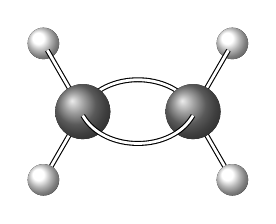
\begin{tikzpicture}[scale=1.0]
  % \useasboundingbox(-2,-1)rectangle(2,1);
  \fill[ball color=white]([shift=(120:1.0)]-0.7,0)circle(0.2);
  \fill[ball color=white]([shift=( 60:1.0)] 0.7,0)circle(0.2);
  \draw[double,double distance=1pt](-0.7,0)--++(120:0.9)(-0.7,0)--++(240:1.0);
  \draw[double,double distance=1pt](0.7,0)--++(60:0.9)(0.7,0)--++(-60:1.0);
  \draw[double,double distance=1pt](-0.7,0.05)to[out=60,in=120](0.7,0.05);
  \fill[ball color=white]([shift=(240:1.0)]-0.7,0)circle(0.2);
  \fill[ball color=white]([shift=(-60:1.0)] 0.7,0)circle(0.2);
  \fill[ball color=gray](-0.7,0)circle(0.35);
  \fill[ball color=gray](0.7,0)circle(0.35);
  \draw[double,double distance=1pt](-0.7,-0.05)to[out=-60,in=-120](0.7,-0.05);
\end{tikzpicture}
\end{document}